% Options for packages loaded elsewhere
\PassOptionsToPackage{unicode}{hyperref}
\PassOptionsToPackage{hyphens}{url}
%
\documentclass[
]{article}
\usepackage{amsmath,amssymb}
\usepackage{lmodern}
\usepackage{iftex}
\ifPDFTeX
  \usepackage[T1]{fontenc}
  \usepackage[utf8]{inputenc}
  \usepackage{textcomp} % provide euro and other symbols
\else % if luatex or xetex
  \usepackage{unicode-math}
  \defaultfontfeatures{Scale=MatchLowercase}
  \defaultfontfeatures[\rmfamily]{Ligatures=TeX,Scale=1}
\fi
% Use upquote if available, for straight quotes in verbatim environments
\IfFileExists{upquote.sty}{\usepackage{upquote}}{}
\IfFileExists{microtype.sty}{% use microtype if available
  \usepackage[]{microtype}
  \UseMicrotypeSet[protrusion]{basicmath} % disable protrusion for tt fonts
}{}
\makeatletter
\@ifundefined{KOMAClassName}{% if non-KOMA class
  \IfFileExists{parskip.sty}{%
    \usepackage{parskip}
  }{% else
    \setlength{\parindent}{0pt}
    \setlength{\parskip}{6pt plus 2pt minus 1pt}}
}{% if KOMA class
  \KOMAoptions{parskip=half}}
\makeatother
\usepackage{xcolor}
\usepackage[margin=1in]{geometry}
\usepackage{graphicx}
\makeatletter
\def\maxwidth{\ifdim\Gin@nat@width>\linewidth\linewidth\else\Gin@nat@width\fi}
\def\maxheight{\ifdim\Gin@nat@height>\textheight\textheight\else\Gin@nat@height\fi}
\makeatother
% Scale images if necessary, so that they will not overflow the page
% margins by default, and it is still possible to overwrite the defaults
% using explicit options in \includegraphics[width, height, ...]{}
\setkeys{Gin}{width=\maxwidth,height=\maxheight,keepaspectratio}
% Set default figure placement to htbp
\makeatletter
\def\fps@figure{htbp}
\makeatother
\setlength{\emergencystretch}{3em} % prevent overfull lines
\providecommand{\tightlist}{%
  \setlength{\itemsep}{0pt}\setlength{\parskip}{0pt}}
\setcounter{secnumdepth}{-\maxdimen} % remove section numbering
\usepackage{booktabs}
\usepackage{longtable}
\usepackage{array}
\usepackage{multirow}
\usepackage{wrapfig}
\usepackage{float}
\usepackage{colortbl}
\usepackage{pdflscape}
\usepackage{tabu}
\usepackage{threeparttable}
\usepackage{threeparttablex}
\usepackage[normalem]{ulem}
\usepackage{makecell}
\usepackage{xcolor}
\ifLuaTeX
  \usepackage{selnolig}  % disable illegal ligatures
\fi
\IfFileExists{bookmark.sty}{\usepackage{bookmark}}{\usepackage{hyperref}}
\IfFileExists{xurl.sty}{\usepackage{xurl}}{} % add URL line breaks if available
\urlstyle{same} % disable monospaced font for URLs
\hypersetup{
  pdftitle={South Sudan},
  hidelinks,
  pdfcreator={LaTeX via pandoc}}

\title{South Sudan}
\author{}
\date{\vspace{-2.5em}}

\begin{document}
\maketitle

\hypertarget{rix-spotlight-for-humanitarian-needs-overview}{%
\subsection{RiX Spotlight for Humanitarian Needs
Overview}\label{rix-spotlight-for-humanitarian-needs-overview}}

\begin{flushright}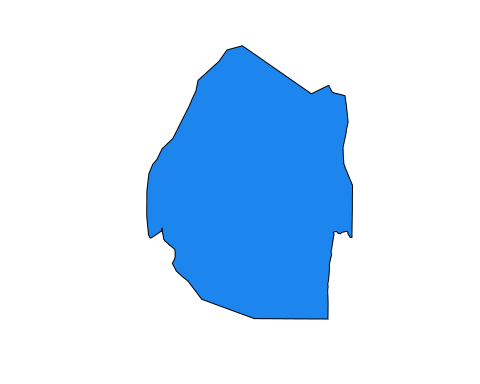
\includegraphics[width=0.2\linewidth]{Spotlight_files/figure-latex/unnamed-chunk-3-1} \end{flushright}

\begin{tabu} to \linewidth {>{\raggedright}X>{\raggedleft}X>{\raggedleft}X>{\raggedright}X>{\raggedleft}X>{\raggedright}X>{\raggedright}X}
\hline
\multicolumn{7}{c}{\bgroup\fontsize{medium}{NA}\selectfont Basic Risk Data\egroup{}} \\
\cline{1-7}
Indicator.Name & Value & Rank & Description & Year & Class_levels & Source\\
\hline
\multicolumn{7}{l}{\textbf{a) Risk Index}}\\
\hline
\hspace{1em}Inform Risk & 8.50 & 2 &  & 2022 & <span style="display: block; padding: 0 4px; border-radius: 4px; background-color: #ee2c2c">Very High</span> & DRMKC INFORM, Mid 2022\\
\hline
\multicolumn{7}{l}{\textbf{b) Hazards \& Exposure}}\\
\hline
\hspace{1em}Hazards & Exposure & 7.30 & 18 &  & 2022 & <span style="display: block; padding: 0 4px; border-radius: 4px; background-color: #ee2c2c">Very High</span> & DRMKC INFORM, Mid 2022\\
\hline
\hspace{1em}Human Hazards & 9.00 & 16 &  & 2022 & <span style="display: block; padding: 0 4px; border-radius: 4px; background-color: #ee2c2c">Very High</span> & DRMKC INFORM, Mid 2022\\
\hline
\hspace{1em}Conflict Barometer & 9.00 & 16 &  & 2022 & <span style="display: block; padding: 0 4px; border-radius: 4px; background-color: #ee8457">High     </span> & DRMKC INFORM, Mid 2022\\
\hline
\hspace{1em}Natural Hazards & 4.10 & 101 &  & 2022 & <span style="display: block; padding: 0 4px; border-radius: 4px; background-color: #eedc82">Moderate </span> & DRMKC INFORM, Mid 2022\\
\hline
\hspace{1em}Agriculture drought probability & 3.50 & 108 &  & 2022 & <span style="display: block; padding: 0 4px; border-radius: 4px; background-color: #eedc82">Moderate </span> & DRMKC INFORM, Mid 2022\\
\hline
\hspace{1em}Exposure to Epidemics & 7.30 & 9 &  & 2022 & <span style="display: block; padding: 0 4px; border-radius: 4px; background-color: #ee2c2c">Very High</span> & DRMKC INFORM, Mid 2022\\
\hline
\hspace{1em}Physical exposure to  earthquake & 2.80 & 107 &  & 2022 & <span style="display: block; padding: 0 4px; border-radius: 4px; background-color: #eedc82">Moderate </span> & DRMKC INFORM, Mid 2022\\
\hline
\hspace{1em}Physical exposure to flood & 7.10 & 33 &  & 2022 & <span style="display: block; padding: 0 4px; border-radius: 4px; background-color: #ee2c2c">Very High</span> & DRMKC INFORM, Mid 2022\\
\hline
\hspace{1em}Forest area (% of land) & 11.33 & 158 &  & 2020 & <span style="display: block; padding: 0 4px; border-radius: 4px; background-color: #88b351">Low      </span> & Food and Agriculture Organization, electronic files and web site.\\
\hline
\hspace{1em}Average precipitation in depth (mm per year) & 900.00 & 99 &  & 2018 & <span style="display: block; padding: 0 4px; border-radius: 4px; background-color: #eedc82">Moderate </span> & Food and Agriculture Organization, electronic files and web site.\\
\hline
\hspace{1em}PM2.5 air pollution, mean annual exposure (micrograms per cubic meter) & 45.58 & 27 &  & 2017 & <span style="display: block; padding: 0 4px; border-radius: 4px; background-color: #ee2c2c">Very High</span> & Brauer, M. et al. 2017, for the Global Burden of Disease Study 2017.\\
\hline
\multicolumn{7}{l}{\textbf{c) Vulnerability}}\\
\hline
\hspace{1em}Vulnerability & 9.00 & 1 &  & 2022 & <span style="display: block; padding: 0 4px; border-radius: 4px; background-color: #ee2c2c">Very High</span> & DRMKC INFORM, Mid 2022\\
\hline
\hspace{1em}Social-Economics Vulnerability & 8.60 & 1 &  & 2022 & <span style="display: block; padding: 0 4px; border-radius: 4px; background-color: #ee2c2c">Very High</span> & DRMKC INFORM, Mid 2022\\
\hline
\hspace{1em}Public aid per capita & 10.00 & 1 &  & 2022 & <span style="display: block; padding: 0 4px; border-radius: 4px; background-color: #ee2c2c">Very High</span> & DRMKC INFORM, Mid 2022\\
\hline
\hspace{1em}Income Gini coefficient - Inequality in income or consumption & 4.80 & 67 &  & 2022 & <span style="display: block; padding: 0 4px; border-radius: 4px; background-color: #ee8457">High     </span> & DRMKC INFORM, Mid 2022\\
\hline
\hspace{1em}Multidimensional Poverty Index & 9.70 & 5 &  & 2022 & <span style="display: block; padding: 0 4px; border-radius: 4px; background-color: #ee2c2c">Very High</span> & DRMKC INFORM, Mid 2022\\
\hline
\hspace{1em}Vulnerable Groups & 9.30 & 2 &  & 2022 & <span style="display: block; padding: 0 4px; border-radius: 4px; background-color: #ee2c2c">Very High</span> & DRMKC INFORM, Mid 2022\\
\hline
\hspace{1em}Adult Prevalence of HIV-AIDS & 8.00 & 3 &  & 2022 & <span style="display: block; padding: 0 4px; border-radius: 4px; background-color: #ee2c2c">Very High</span> & DRMKC INFORM, Mid 2022\\
\hline
\hspace{1em}Returned refugees & 10.00 & 7 &  & 2022 & <span style="display: block; padding: 0 4px; border-radius: 4px; background-color: #ee2c2c">Very High</span> & DRMKC INFORM, Mid 2022\\
\hline
\hspace{1em}Mortality rate under 5 (per 1K births) & 97.90 & 6 &  & 2020 & <span style="display: block; padding: 0 4px; border-radius: 4px; background-color: #ee2c2c">Very High</span> & Estimates developed by the UN Inter-agency Group for Child Mortality Estimation (UNICEF, WHO, World Bank, UN DESA Population Division) at www.childmortality.org.\\
\hline
\hspace{1em}Vulnerable employment (% of total employment) & 90.24 & 6 &  & 2019 & <span style="display: block; padding: 0 4px; border-radius: 4px; background-color: #ee2c2c">Very High</span> & Derived using data from International Labour Organization, ILOSTAT database.\\
\hline
\multicolumn{7}{l}{\textbf{d) Lack fo Coping Capacity}}\\
\hline
\hspace{1em}Lack of Coping Capacity & 9.50 & 1 &  & 2022 & <span style="display: block; padding: 0 4px; border-radius: 4px; background-color: #ee2c2c">Very High</span> & DRMKC INFORM, Mid 2022\\
\hline
\hspace{1em}Infrastructural Lack of Coping Capacity & 9.70 & 1 &  & 2022 & <span style="display: block; padding: 0 4px; border-radius: 4px; background-color: #ee2c2c">Very High</span> & DRMKC INFORM, Mid 2022\\
\hline
\hspace{1em}Maternal Mortality Ratio & 9.80 & 1 &  & 2022 & <span style="display: block; padding: 0 4px; border-radius: 4px; background-color: #ee2c2c">Very High</span> & DRMKC INFORM, Mid 2022\\
\hline
\hspace{1em}Mobile celluar subscriptions & 9.40 & 1 &  & 2022 & <span style="display: block; padding: 0 4px; border-radius: 4px; background-color: #ee2c2c">Very High</span> & DRMKC INFORM, Mid 2022\\
\hline
\hspace{1em}Improved sanitation facilities & 9.80 & 4 &  & 2022 & <span style="display: block; padding: 0 4px; border-radius: 4px; background-color: #ee2c2c">Very High</span> & DRMKC INFORM, Mid 2022\\
\hline
\hspace{1em}Institutional Lack of Coping Capacity & 9.30 & 1 &  & 2022 & <span style="display: block; padding: 0 4px; border-radius: 4px; background-color: #ee2c2c">Very High</span> & DRMKC INFORM, Mid 2022\\
\hline
\hspace{1em}Corruption Perception Index & 9.30 & 1 &  & 2022 & <span style="display: block; padding: 0 4px; border-radius: 4px; background-color: #ee2c2c">Very High</span> & DRMKC INFORM, Mid 2022\\
\hline
Food production index & 102.53 & 117 &  & 2020 & <span style="display: block; padding: 0 4px; border-radius: 4px; background-color: #eedc82">Moderate </span> & Food and Agriculture Organization, electronic files and web site.\\
\hline
Human Capital Index (HCI) (scale 0-1) & 0.31 & 171 &  & 2020 & <span style="display: block; padding: 0 4px; border-radius: 4px; background-color: #228b22">Very Low </span> & World Bank staff calculations based on the methodology described in World Bank (2018). https://openknowledge.worldbank.org/handle/10986/30498\\
\hline
Ease of doing business score (0 = lowest performance to 100 = best performance) & 34.62 & 185 &  & 2019 & <span style="display: block; padding: 0 4px; border-radius: 4px; background-color: #228b22">Very Low </span> & World Bank, Doing Business project (http://www.doingbusiness.org/). NOTE: Doing Business has been discontinued as of 9/16/2021. For more information: https://bit.ly/3CLCbme\\
\hline
Unemployment, female (% of female labor force) (modeled ILO estimate) & 15.26 & 42 &  & 2021 & <span style="display: block; padding: 0 4px; border-radius: 4px; background-color: #ee8457">High     </span> & International Labour Organization, ILOSTAT database. Data as of June 2022.\\
\hline
Unemployment, male (% of male labor force) (modeled ILO estimate) & 12.61 & 30 &  & 2021 & <span style="display: block; padding: 0 4px; border-radius: 4px; background-color: #ee2c2c">Very High</span> & International Labour Organization, ILOSTAT database. Data as of June 2022.\\
\hline
Net migration & -870998.00 & 188 &  & 2017 & <span style="display: block; padding: 0 4px; border-radius: 4px; background-color: #228b22">Very Low </span> & United Nations Population Division. World Population Prospects: 2019 Revision.\\
\hline
Rural population (% of population) & 79.49 & 10 &  & 2021 & <span style="display: block; padding: 0 4px; border-radius: 4px; background-color: #ee2c2c">Very High</span> & World Bank staff estimates based on the United Nations Population Division's World Urbanization Prospects: 2018 Revision.\\
\hline
\end{tabu}

\begin{tabu} to \linewidth {>{\raggedright}X>{\raggedleft}X}
\hline
\multicolumn{2}{c}{\bgroup\fontsize{medium}{NA}\selectfont Country Statistics\egroup{}} \\
\cline{1-2}
Description & Mean Value\\
\hline
Population & 143463.44\\
\hline
Female Population & 71645.71\\
\hline
Under 14 Population & 58920.72\\
\hline
Over 64 Population & 4825.29\\
\hline
GDP-PPP Per Capita (USD-2011) & 3927.49\\
\hline
Air Pollution (micrograms/m^3) & 22.48\\
\hline
Flood Risk: 100 Year Return Period & 2.52\\
\hline
Drought Risk: 50 Year Return Period & 5110.80\\
\hline
Earthquake Risk: 475 Year Return Period & 39.51\\
\hline
Landslide Risk & 0.00\\
\hline
Extreme Heat Risk: 20 Year Return Period & 31.03\\
\hline
Tsunami Risk & NA\\
\hline
Subnational Human Development Index & 0.38\\
\hline
Health Index & 0.59\\
\hline
Living Standards Index & 0.34\\
\hline
Education Index & 0.28\\
\hline
Life Expectancy (years) & 58.49\\
\hline
Gross National Income (USD-2011) & 985.28\\
\hline
Expected Schooling Years & 4.81\\
\hline
Mean Schooling Years & 4.47\\
\hline
Projected Precipitation Difference 2022-2050 & 0.00\\
\hline
Projected Surface Temperature Difference 2022-2050 & 0.75\\
\hline
Projected Total Runoff Difference 2022-2050 & NA\\
\hline
Projected: Maximum Consecutive Dry Days & 8.38\\
\hline
Projected: Maximum Consecutive Wet Days & 64.35\\
\hline
Projected: Length of Growing Season & 365.00\\
\hline
Projected: Annual Minimum Daily Minimum Temperature (Celsius) & 24.36\\
\hline
Projected: Annual Maximum Daily Maximum Temperature (Celsius) & 29.37\\
\hline
\end{tabu}

\end{document}
